\chapter{Layered Editor Architectures}
\label{chap:layeredArchs}
{\em *** Version: \today~ ***}


\bc

IMPORTANT there seems to be an invariant that for a j:  i>j, all mappings are correct 
  ..           ...       
 .  .    ..   .   .   .. 
.    ....  ...     ...  .
no it's not asymmetric. find out more about this.
maybe it's just that a level is never presented twice without intr, and vice versa


MAYBE DO SOME NON layered stuff first? to explain what spec. will mean. more important if things like intention of edit op is added as an equation.
\ec

% intro

\bc
Using the single layer specification from the previous chapter, we can give a specification for a layered editor architecture. The building blocks for the specification are . The specification for a single layer from the previous chapterprev. chap. spec for layer but not edit and transform. Edit result in new lower level, initiated by gesture from user. Transform higher. In this chapter,level take all layers together and combine. At top and bottom, some extra stuff.
\ec

\bl
\* Spec for editor is combined spec for single layers.
\* abstract $\Edit$ and $\Transform$ removed
\* Next chapter, we give Haskell for the combination.
\el

\bl
\* In this chapter, combine the single layer specifications.
\* First combine everything, assuming edit ops are indirect (ref Chapter Edit Model)
\* Section~\ref{sect:specHigherEdit} support for direct interpretation of edit ops
\* Section~\ref{sect:specSkipLayers} support for skipping higher layers
\el

\fromHere  % VVVVVVVVVVVVVVVVVVVVVVVVVVVVVVVVVVVVVVVVVVVV

\section{Specifying a layered editor}\label{sect:specCombination}

The starting point for the specification of a layerer editor is the incremental specification of a single layer, given in Section~\ref{sect:maintainingInc} of the previous chapter. The layered specification consists of a combination of several instances of the single layer specification. Before we combine the layers, we first give an informal sketch of the combination process.

\subsection{Combining layers}
\note{Add arrow stating that the result is what we mean with the gesture? (eg. $\level''_n = Intended~e_{\Level_n}~\level_n~(\dots \level_0)$)}

Figure~\ref{singleToMulti1} shows a simplified version of the final figure (Figure~\ref{maintainExtraState}) from Section~\ref{sect:maintainingInc}. Except for the level updates, all internal data flow is hidden, showing only the input and output values of the level. The updates are not hidden, because some updates need to be removed when combining layers.\note{first explain non-layered situation? Or is this clear enough?}

\begin{figure}[h]
  \hfill
  \begin{minipage}[b]{.45\textwidth}
    \begin{center}  
      \epsfig{file=pics/eps/singleToMulti1.eps, width = 60mm}
      \caption{A single layer.} \label{singleToMulti1}
    \end{center}
  \end{minipage}
  \hfill
  \begin{minipage}[b]{.45\textwidth}
    \begin{center}  
      \epsfig{file=pics/eps/singleToMulti2.eps, width = 60mm}\\ \vspace{0.765cm}
      \caption{$Layer_i$.} \label{singleToMulti2}
    \end{center}
  \end{minipage}
  \hfill
\end{figure}

\bigskip
{\bf Replacing $H$ and $L$:}

To be able to combine multiple layers, the $H$ and $L$ subscripts are replaced by natural numbers. Because the document is $\level_0$, and the rendering is $\level_n$, a higher level gets an index $i$ whereas a lower level gets an index $i+1$. The functions $\interpret$ and $\present$ get a subscript $i$. Figure~\ref{singleToMulti2} contains the resulting indexed layer. 

Note that the abstract functions $\Edit$ and $\Transform$ have been dropped because except at the top and bottom, adjacent layers will now take care of this functionality. At the end of this section, we explain how the situation at the top and the bottom is dealt with.

\bigskip
{\bf Dropping superfluous updates:} 

The layer in Figure~\ref{singleToMulti2} is not ready to be combined yet, because it because on interpretation and presentation, it updates both the upper level ($i$) and the lower level ($i+1$). Hence, if it is combined with an adjacent layer, the level in between is updated twice on interpretation, and twice on presentation. Therefore, we drop one update in the interpration phase and one in the presentation phase. 

In order to decide which update to drop, recall that Section~\ref{sect:incrementalSpec} explained that an implementation of a mapping function may perform an update on the source level of the mapping. Thus, 
$\interpret$ may update the lower level, and $\present$ may update the higher level. In order to still allow this behavior, we choose to drop the updates on the target levels: the higher level update in the interpretation phase (upper left dotted arrow), and the lower level update in the presentation phase (lower right dotted arrow). 

Figure~\ref{combiningLayers1} shows a layer after the two target level update are dropped. When the layer is combined, the dropped target level updates are performed by an adjacent layer, except at the top and the bottom where we need to handle the updates explicitly. Figure~\ref{combiningLayers2} shows a combination of several layers.

\begin{figure}[h]
  \hfill
  \begin{minipage}[b]{.45\textwidth}
    \begin{center}  
      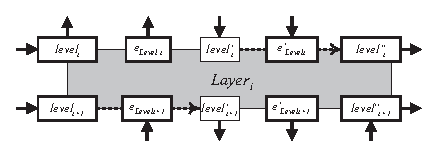
\epsfig{file=pics/eps/connectingLayers1.eps, width = 60mm}
      \caption{Layer $i$ with two updates.} \label{combiningLayers1}
    \end{center}
  \end{minipage}
  \hfill
  \begin{minipage}[b]{.45\textwidth}
    \begin{center}  
      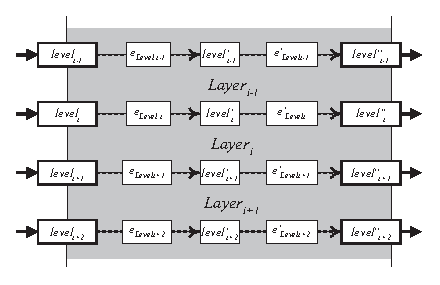
\epsfig{file=pics/eps/connectingLayers2.eps, width = 60mm}
      \caption{Combined layers.} \label{combiningLayers2}
    \end{center}
  \end{minipage}
  \hfill
\end{figure}


\bigskip
{\bf Handling the top and bottom:}

The combination in Figure~\ref{combiningLayers2}, shows what happens for internal layers that are surrounded by other layers. However at the top and the bottom of the layered architecture, still some work needs to be done, because of the missing $\Edit$ and $\Transform$ functions and the dropped updates. 

At the top, edit operations coming out of the interpretation phase need to be put back into the presentation phase. And at the bottom, an edit gesture from the user must be put into the combined layers combination, and an updated rendering must be shown to the user. The left-hand side of Figure~\ref{topAndBottom} shows the loose ends that need to be dealt with.

\begin{figure}\begin{center}\begin{center}
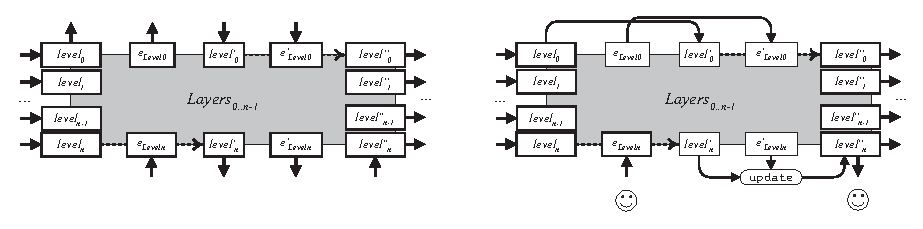
\epsfig{file=pics/eps/topAndBottom.eps, width=125mm}\end{center}
\caption{Loose ends at the top and bottom vs. final dataflow}\label{topAndBottom} 
\end{center}\end{figure}\note{TODO: add dotted line between level1 and n-1}

\note{gesture depends on level, not edit. Also on other levels?}

At the top, the result of the combined interpret mappings is a document edit operation $e_{\Level_0}$. Because the target update of each layer has been dropped, the operation is not performed on the document $\level_0$. Furthermore, due to the missing $\Transform$ we need to specify how to get from $e_{\Level_0}$ to $e'_{\Level_0}$. Rather than explicitly adding an update on $\level_0$, we put the level and the edit operation back into the presentation part of the combined layers. This way, the document update is performed by the presentation phase of the top layer.

Similar to the top, the bottom also misses an update. Therefore, we add an update at the bottom right, which applies $e'_{\Level_n}$ to $\level'_n$. For sake of clarity, we use the explicit notation rather than a dashed arrow. 

Finally, because of the missing $\Edit$, we need to specify how the edit gesture from the user is to be fed into the layer structure, and how the updated lower level is to be shown to the user. The right-hand side of Figure~\ref{topAndBottom} shows the data flow at the top and the bottom of the layers. Note that $\level''_n$ has both an incoming arrow from the update, as well as an outgoing arrow symbolizing that the rendering is shown to the user.

\subsection{Specifying combined layers}

We construct the specification of the combined layers along the same lines as in the previous section. Recall that the data level definitions from a multiple layer perspective (see Section~\ref{sect:mappingInformation}) are:

\begin{small}\( \begin{array}{lcl}  \label{inv:incrementality}
\text{\bf type}~\Level_{0}  =  \Core_{\Intr,0} \times \Extra_{\Intr,0} \times \Info\idwn_{0} \\
\text{\bf type}~\Level_{n}  =  \Core_{\Pres,n} \times \Extra_{\Pres,n} \times  \Info\iup_{n}\\
\lefteqn{\forall j:1 \le j \le n-1:}  \\
\text{\bf type}~\Level_{j} =  \Core_{\Pres,j} \times \Extra_{\Pres,j}  \times \Info\iup_{j}   
                                       =  \Core_{\Intr,j} \times \Extra_{\Intr,j} \times \Info\idwn_{j}
\end{array}\)\end{small}

\bigskip
{\bf Replacing $H$ and $L$:}

First, we take the  final single layer specification from Section~\ref{sect:maintainingInc}, and replace the $H$ and $L$ subscripts by $i$ and $i+1$. Except for $\update$, the values and functions without an $H$ or $L$ subscript in specification~\ref{spec:incrementality} ($\sheet$, $\interpret$, $\present$, and
 $\reuse$) are now specific to a certain layer and get an $i$ subscript. Because $\update$ is a generic function it can be used in all layers without a subscript. Finally, because we specify all layers instead of just a single one, we no longer need the $\Edit$ and $\Transform$ equations for describing the behavior of adjacent layers.

\begin{small}
\refstepcounter{specification} \label{spec:combinationFirstAttempt}
\( \begin{array}{rcll}  
{\tt interpret_i}  & :: & \multicolumn{2}{l}{\Sheet_{\Intr,i} \rightarrow \Level_{i+1} \rightarrow \Level_{i} \rightarrow  \Edit_{\Level_{i+1}} \rightarrow \Edit_{\Core_{i}\times \Info\idwn_{i}} } \\
{\tt present_i} & :: & \multicolumn{2}{l}{ \Sheet_{\Pres,i} \rightarrow \Level_{i} \rightarrow \Level_{i+1}  \rightarrow \Edit_{\Level_{i}} \rightarrow \Edit_{\Core_{i+1}\times \Info\iup_{i+1}} } \\
\level_{i+1} 	& = & \Present_{i}~\level_{i}						& \text{\{Precondition\}}\\
\\
\level'_{i+1} 	& = & \update~e_{\Level_{i+1}}~\level_{i+1}                 & \text{\{Compute intermediate lower level\}}\\
e_{\Core_{i} \times \Info\idwn_{i}}  & = & \interpret_{i}~\sheet_{\Intr,i}~\level_{i+1}~\level_{i}~e_{\Level_{i+1}} & \text{\{Compute higher core update\}}\\
e_{\Level_{i}} & = & \reuse_{\Intr,i}~\level_{i}~e_{\Core_{i}\times \Info\idwn_{i}}     & \text{\{Reuse extra state\}}\\
\level'_{i} & = & \update~e_{\Level_{i}}~\level_{i}                 & \text{\{Compute intermediate higher level\}}\\
\\\
\level'_{i} & = & \Interpret_{i}~\level'_{i+1}						& \text{\{Intermediate condition\}}\\
\\
\level''_{i} & = & \update~e'_{\Level_{i}}~\level'_{i}                 & \text{\{Compute final higher level\}}\\
e'_{\Core_{i+1}\times \Info\iup_{i+1}}  & = & \present_{i}~\sheet_{\Pres,i}~\level'_{i}~\level'_{i+1}~e'{\Level_{i}} & \text{\{Compute new lower core\}}\\
e'_{\Level_{i+1}} & = & \reuse_{\Pres,i}~\level_{i+1}~e'_{\Core_{i+1}\times \Info\iup_{i+1}} & \text{\{Reuse extra state\}}\\
\level''_{i+1} & = & \update~e_{\Level_{i+1}}~\level_{i+1}                 & \text{\{Compute final lower level\}}\\
\\
\level''_{i+1} & = & \Present_{i}~\level''_{i}						& \text{\{Postcondition\}}\\
\end{array}\)
\end{small}
\begin{center}(Specification \thespecification: First attempt)\end{center}\vspace{1em}

\note{what to do about levels and layers subscript mismatch layers 0..n-1 levels 0..n-1? Just use $i$ and $j$?}

\bigskip
{\bf Dropping superfluous updates:}

The specification has double updates on all levels except the document and the rendering, because updates for $\level$ and $\level'$ are specified on the higher level $i$ as well as the lower level $i+1$. This problem has been solved in the previous section by dropping the updates on the target levels (equations \{Compute intermediate higher level\} and \{Compute final lower level\}). The remaining updates are:

\begin{small}\( \begin{array}{lcll} 
\level'_{i+1} 	& = & \update~e_{\Level_{i+1}}~\level_{i+1}                 & \text{\{Compute intermediate lower level\}}\\
\level''_{i} & = & \update~e'_{\Level_{i}}~\level'_{i}                 & \text{\{Compute final higher level\}}\\
\end{array}\)
\end{small}

\bigskip
{\bf Handling the top and bottom:}

Due to the dropped updates, there are no computations for $\level'_0$ and $\level''{n}$. And moreover, $e_{\Level_n}$ and $e'_{\Level_0}$ need to be defined, since $\Edit$ and $\Transform$ have been dropped. 

At the top, the document and the edit operation on it ($\level_0$ and $e_{\Level_0}$) are put back into the computation by assigning them to $\level'_0$ and $e'_{\Level_0}$, yielding:

\begin{small}\( \begin{array}{lcll} 
e'_{\Level_{0}}  & = & e_{\Level_{0}}		& \text{\{?\}}\\
\level'_{0} & = & \level_{0}				& \text{\{?\}}\\
\end{array}\)
\end{small}

At the bottom, we add a rendering update on $\level'_n$ and specify that $e_{\Level_n}$ is the edit gesture that comes from the user. The fact that the updated rendering $\level''_n$ is shown to the user is not explicitly visible in the specification.\note{how to encode EditGesture?}

\begin{small}\( \begin{array}{lcll} 
e_{\Level_{n}} & = & \mathit{EditGesture} ??		& \text{\{Receive edit gesture\}}\\
\level''_{n}  & = & \update~e'_{\Level_{n}}~\level'_{n}	& \text{\{Update rendering\}}\\
\end{array}\)
\end{small}

\bigskip
{\bf Final specification:}

If we remove the double updates and add the equations for handling the top and bottom cases, we get the final specification: \note{how to layout this thing?}

\begin{small}
\refstepcounter{specification} \label{spec:combination}
\( \begin{array}{lcl} 
\text{\bf type}~\Level_{0}  =  \Core_{\Intr,0} \times \Extra_{\Intr,0} \times \Info\idwn_{0} \\
\text{\bf type}~\Level_{n}  =  \Core_{\Pres,n} \times \Extra_{\Pres,n} \times  \Info\iup_{n}\\
\lefteqn{\forall j:1 \le j \le n-1:}  \\
\text{\bf type}~\Level_{j} =  \Core_{\Pres,j} \times \Extra_{\Pres,j}  \times \Info\iup_{j}   
                                       =  \Core_{\Intr,j} \times \Extra_{\Intr,j} \times \Info\idwn_{j}\\
\\
\lefteqn{\forall i:0 \le i \le n-1:}  \\
\end{array}\) \\
\( \begin{array}{rcll}  
{\tt interpret_i}  & :: & \multicolumn{2}{l}{ \Sheet_{\Intr,i} \rightarrow \Level_{i+1} \rightarrow \Level_{i} \rightarrow  \Edit_{\Level_{i+1}} \rightarrow \Edit_{\Core_{i}\times \Info\idwn_{i}} } \\
{\tt present_i} & :: &  \multicolumn{2}{l}{ \Sheet_{\Pres,i} \rightarrow \Level_{i} \rightarrow \Level_{i+1}  \rightarrow \Edit_{\Level_{i}} \rightarrow \Edit_{\Core_{i+1}\times \Info\iup_{i+1}} } \\
\\
e_{\Level_{n}}  & = & \mathit{EditGesture} ??		& \text{\{Receive edit gesture\}}\\
e'_{\Level_{0}}  & = & e_{\Level_{0}}		& \text{\{?\}}\\
\level'_{0} & = & \level_{0}				& \text{\{?\}}\\
\level''_{n}  & = & \update~e'_{\Level_{n}}~\level'_{n}			& \text{\{Update rendering\}}\\
\level_{i+1} 	& = & \Present_{i}~\level_{i}						& \text{\{Precondition\}}\\
\\
\level'_{i+1} 	& = & \update~e_{\Level_{i+1}}~\level_{i+1}                 & \text{\{Compute intermediate lower level\}}\\
e_{\Core_{i} \times \Info\idwn_{i}}  & = & \interpret_{i}~\sheet_{\Intr,i}~\level_{i+1}~\level_{i}~e_{\Level_{i+1}} & \text{\{Compute higher core update\}}\\
e_{\Level_{i}} & = & \reuse_{\Intr,i}~\level_{i}~e_{\Core_{i}\times \Info\idwn_{i}}     & \text{\{Reuse extra state\}}\\
\\
\level'_{i} & = & \Interpret_{i}~\level'_{i+1}						& \text{\{Intermediate condition\}}\\
\\
\level''_{i} & = & \update~e'_{\Level_{i}}~\level'_{i}                 & \text{\{Compute final higher level\}}\\
e'_{\Core_{i+1}\times \Info\iup_{i+1}}  & = & \present_{i}~\sheet_{\Pres,i}~\level'_{i}~\level'_{i+1}~e'{\Level_{i}} & \text{\{Compute new lower core\}}\\
e'_{\Level_{i+1}} & = & \reuse_{\Pres,i}~\level_{i+1}~e'_{\Core_{i+1}\times \Info\iup_{i+1}} & \text{\{Reuse extra state\}}\\
\\
\level''_{i+1} & = & \Present_{i}~\level''_{i}						& \text{\{Postcondition\}}\\
\end{array}\)
\end{small}
\begin{center}(Specification \thespecification: Final specification)\end{center}\vspace{1em}

The specification describes the behavior of the editor for a single edit step. The state of the editor is formed by all data levels together ($\Level_{0\dots n}$). ***

Given an initial state ($\level_{0\dots n}$) for which the {\em Presentation} invariant holds, and an edit gesture from a user, the specification describes what values need to be computed in order to yield the state of the editor after the edit gesture is applied ($\level''_{0\dots n}$). The new state is the initial state for the next edit step.

The editor application is started with empty values for each of the levels, between which the {\em Presentation} invariant holds by default. The first edit gesture will be an operation that either loads a document, or creates a new one, after which the normal editing process can start.


%																
%																
%																
\section{Edit operations  on higher levels} \label{sect:specHigherEdit}

Until now, the specification in this chapter assumed an indirect interpretation of edit operations (see Section~\ref{sect:intrProcess}). In other words, a user is assumed to edit the lowest level (the rendering or $\Level_n$), which is then interpreted to yield a new $\Level_{n-1}$. Subsequently, the new $\Level_{n-1}$ is interpreted, yielding a new $\Level_{n-2}$, and the process is continued until the document level ($\Level_0$). However, as we pointed out in Chapter~\ref{chap:proxArch}, this is exactly not how interpretation takes place.\note{Problem with direct/indirect terminology}

\toHere     % ^^^^^^^^^^^^^^^^^^^^^^^^^^^^^^^^^^^^^

Instead of editing the rendering, an edit operation targets one of the higher levels (Layout, Enriched document, or Document). Below that level, the edit operation is interpreted directly (without being applied to any data levels), and from the targeted level upward, the indirect interpretation process takes over.

So target a level j: direct translation of edit op (not affecting levels), after which indirect interpretation takes place.

\bl
\* consequences for es safety
\* lower are not just skips, but direct edit op interpretations.
\* tricky. maybe need to point out diff between skipping and processing
\* kind of phase shift. Entire translation/presentation process is completed, but it starts at higher translation and also ends there.
\el

\bl
\* trans . pres = id so levels stay the same. Only reason for translating is info.
\el

Spec:

\bl
\* edit op on level $j$ (== higher level for layer $j$)
\* $\forall i\le j:$ original spec. holds
\* $\forall i>j: e_j = skip$ 
\* $\level'_j = Translate_j~\level'_{j+1}$ does not hold $\level''_{j+1} = \Present_j~\level''_j$ does
\* After edit op, need to translate at layers $n\dots j$ for mapping info.
\el 

\section{Skipping higher layers} \label{sect:specSkipLayers}

The last adjustment we make to the specification is 

\bl
\* ref to edit model chapter. Chapter~\ref{chap:editModel}
\* layered arch offer a way to skip certain things during editing.
\* kind of optimization, but also desired behavior
\* computed values changing for intermediate doc instances, optimal line breaking. Busy for a user 
\el

\bl
\* skipping cycles + es safety
\* with update on only lower ES, automatic skip, but then no problem with invariants
\* must be careful
\el

Spec:
\bl
\* skipping layers $0\dots j$
\* $\forall i>j:$ original spec. holds
\* $\forall i\le j: e_j and e'_j = skip and e'_{j+1} = e{j+1}$  
\* Invs. still hold, except at skipping point: $Translate_j$ and $\Present_j$ do not hold.
\el

\section{Conclusions}

\bl
\* ?
\el




